\documentclass[12pt,twoside]{article}
\usepackage[dvipsnames]{xcolor}
\usepackage{tikz,graphicx,amsmath,amsfonts,amscd,amssymb,bm,cite,epsfig,epsf,url}
\usepackage[hang,flushmargin]{footmisc}
\usepackage[colorlinks=true,urlcolor=blue,citecolor=blue]{hyperref}
\usepackage{amsthm,multirow,wasysym,appendix}
\usepackage{array,subcaption} 
% \usepackage[small,bf]{caption}
\usepackage{bbm}
\usepackage{pgfplots}
\usetikzlibrary{spy}
\usepgfplotslibrary{external}
\usepgfplotslibrary{fillbetween}
\usetikzlibrary{arrows,automata}
\usepackage{thmtools}
\usepackage{blkarray} 
\usepackage{textcomp}

\usepackage[left=0.8in,right=1.0in,top=1.0in,bottom=1.0in]{geometry}
\newcommand{\red}[1]{{\leavevmode\color{red}{#1}}}
\newcommand{\blue}[1]{{\leavevmode\color{blue}{#1}}}
\usepackage{graphicx}
%% Probability operators and functions
%
% \def \P{\mathrm{P}}
\def \P{\mathrm{P}}
\def \E{\mathrm{E}}
\def \Var{\mathrm{Var}}
\let\var\Var
\def \Cov {\mathrm{Cov}} \let\cov\Cov
\def \MSE {\mathrm{MSE}} \let\mse\MSE
\def \sgn {\mathrm{sgn}}
\def \R {\mathbb{R}}
\def \C {\mathbb{C}}
\def \N {\mathbb{N}}
\def \Z {\mathbb{Z}}
\def \cV {\mathcal{V}}
\def \cS {\mathcal{S}}

\newcommand{\RR}{\ensuremath{\mathbb{R}}}

\DeclareMathOperator*{\argmin}{arg\,min}
\DeclareMathOperator*{\argmax}{arg\,max}
\newcommand{\red}[1]{\textcolor{red}{#1}}
\newcommand{\blue}[1]{\textcolor{blue}{#1}}
\newcommand{\green}[1]{\textcolor{ForestGreen}{ #1}}
\newcommand{\fuchsia}[1]{\textcolor{RoyalPurple}{ #1}}

\newcommand{\wrnd}[1]{\widetilde{ #1 } }
\newcommand{\po}{\wrnd{\op{po}}  }

%
%% Probability distributions
%
%\def \Bern    {\mathrm{Bern}}
%\def \Binom   {\mathrm{Binom}}
%\def \Exp     {\mathrm{Exp}}
%\def \Geom    {\mathrm{Geom}}
% \def \Norm    {\mathcal{N}}
%\def \Poisson {\mathrm{Poisson}}
%\def \Unif    {\mathrm {U}}
%
\DeclareMathOperator{\Norm}{\mathcal{N}}

\newcommand{\bdb}[1]{\textcolor{red}{#1}}

\newcommand{\ml}[1]{\mathcal{ #1 } }
\newcommand{\wh}[1]{\widehat{ #1 } }
\newcommand{\wt}[1]{\widetilde{ #1 } }
\newcommand{\conj}[1]{\overline{ #1 } }
\newcommand{\rnd}[1]{\tilde{ #1 } }
\newcommand{\rv}[1]{ \rnd{ #1}  }
\newcommand{\rM}{\rnd{ m}  }
\newcommand{\rx}{\rnd{ x}  }
\newcommand{\ry}{\rnd{ y}  }
\newcommand{\rz}{\rnd{ z}  }
\newcommand{\ra}{\rnd{ a}  }
\newcommand{\rb}{\rnd{ b}  }
\newcommand{\rt}{\rnd{ t}  }
\newcommand{\rs}{\rnd{ s}  }


\newcommand{\rpc}{\widetilde{ pc}  }
\newcommand{\rndvec}[1]{\vec{\rnd{#1}}}

\def \cnd {\, | \,}
\def \Id { I }
\def \J {\mathbf{1}\mathbf{1}^T}

\newcommand{\op}[1]{\operatorname{#1}}
\newcommand{\setdef}[2]{ := \keys{ #1 \; | \; #2 } }
\newcommand{\set}[2]{ \keys{ #1 \; | \; #2 } }
\newcommand{\sign}[1]{\op{sign}\left( #1 \right) }
\newcommand{\trace}[1]{\op{tr}\left( #1 \right) }
\newcommand{\tr}[1]{\op{tr}\left( #1 \right) }
\newcommand{\inv}[1]{\left( #1 \right)^{-1} }
\newcommand{\abs}[1]{\left| #1 \right|}
\newcommand{\sabs}[1]{| #1 |}
\newcommand{\keys}[1]{\left\{ #1 \right\}}
\newcommand{\sqbr}[1]{\left[ #1 \right]}
\newcommand{\sbrac}[1]{ ( #1 ) }
\newcommand{\brac}[1]{\left( #1 \right) }
\newcommand{\bbrac}[1]{\big( #1 \big) }
\newcommand{\Bbrac}[1]{\Big( #1 \Big)}
\newcommand{\BBbrac}[1]{\BIG( #1 \Big)}
\newcommand{\MAT}[1]{\begin{bmatrix} #1 \end{bmatrix}}
\newcommand{\sMAT}[1]{\left(\begin{smallmatrix} #1 \end{smallmatrix}\right)}
\newcommand{\sMATn}[1]{\begin{smallmatrix} #1 \end{smallmatrix}}
\newcommand{\PROD}[2]{\left \langle #1, #2\right \rangle}
\newcommand{\PRODs}[2]{\langle #1, #2 \rangle}
\newcommand{\der}[2]{\frac{\text{d}#2}{\text{d}#1}}
\newcommand{\pder}[2]{\frac{\partial#2}{\partial#1}}
\newcommand{\derTwo}[2]{\frac{\text{d}^2#2}{\text{d}#1^2}}
\newcommand{\ceil}[1]{\lceil #1 \rceil}
\newcommand{\Imag}[1]{\op{Im}\brac{ #1 }}
\newcommand{\Real}[1]{\op{Re}\brac{ #1 }}
\newcommand{\norm}[1]{\left|\left| #1 \right|\right| }
\newcommand{\norms}[1]{ \| #1 \|  }
\newcommand{\normProd}[1]{\left|\left| #1 \right|\right| _{\PROD{\cdot}{\cdot}} }
\newcommand{\normTwo}[1]{\left|\left| #1 \right|\right| _{2} }
\newcommand{\normTwos}[1]{ \| #1  \| _{2} }
\newcommand{\normZero}[1]{\left|\left| #1 \right|\right| _{0} }
\newcommand{\normTV}[1]{\left|\left| #1 \right|\right|  _{ \op{TV}  } }% _{\op{c} \ell_1} }
\newcommand{\normOne}[1]{\left|\left| #1 \right|\right| _{1} }
\newcommand{\normOnes}[1]{\| #1 \| _{1} }
\newcommand{\normOneTwo}[1]{\left|\left| #1 \right|\right| _{1,2} }
\newcommand{\normF}[1]{\left|\left| #1 \right|\right| _{\op{F}} }
\newcommand{\normLTwo}[1]{\left|\left| #1 \right|\right| _{\ml{L}_2} }
\newcommand{\normNuc}[1]{\left|\left| #1 \right|\right| _{\ast} }
\newcommand{\normOp}[1]{\left|\left| #1 \right|\right|  }
\newcommand{\normInf}[1]{\left|\left| #1 \right|\right| _{\infty}  }
\newcommand{\proj}[1]{\mathcal{P}_{#1} \, }
\newcommand{\diff}[1]{ \, \text{d}#1 }
\newcommand{\vc}[1]{\boldsymbol{\vec{#1}}}
\newcommand{\rc}[1]{\boldsymbol{#1}}
\newcommand{\vx}{\vec{x}}
\newcommand{\vy}{\vec{y}}
\newcommand{\vz}{\vec{z}}
\newcommand{\vu}{\vec{u}}
\newcommand{\vv}{\vec{v}}
\newcommand{\vb}{\vec{\beta}}
\newcommand{\va}{\vec{\alpha}}
\newcommand{\vaa}{\vec{a}}
\newcommand{\vbb}{\vec{b}}
\newcommand{\vg}{\vec{g}}
\newcommand{\vw}{\vec{w}}
\newcommand{\vh}{\vec{h}}
\newcommand{\vbeta}{\vec{\beta}}
\newcommand{\valpha}{\vec{\alpha}}
\newcommand{\vgamma}{\vec{\gamma}}
\newcommand{\veta}{\vec{\eta}}
\newcommand{\vnu}{\vec{\nu}}
\newcommand{\rw}{\rnd{w}}
\newcommand{\rvnu}{\vc{\nu}}
\newcommand{\rvv}{\rndvec{v}}
\newcommand{\rvw}{\rndvec{w}}
\newcommand{\rvx}{\rndvec{x}}
\newcommand{\rvy}{\rndvec{y}}
\newcommand{\rvz}{\rndvec{z}}
\newcommand{\rvX}{\rndvec{X}}


\newtheorem{theorem}{Theorem}[section]
% \declaretheorem[style=plain,qed=$\square$]{theorem}
\newtheorem{corollary}[theorem]{Corollary}
\newtheorem{definition}[theorem]{Definition}
\newtheorem{lemma}[theorem]{Lemma}
\newtheorem{remark}[theorem]{Remark}
\newtheorem{algorithm}[theorem]{Algorithm}

% \theoremstyle{definition}
%\newtheorem{example}[proof]{Example}
\declaretheorem[style=definition,qed=$\triangle$,sibling=definition]{example}
\declaretheorem[style=definition,qed=$\bigcirc$,sibling=definition]{application}

%
%% Typographic tweaks and miscellaneous
%\newcommand{\sfrac}[2]{\mbox{\small$\displaystyle\frac{#1}{#2}$}}
%\newcommand{\suchthat}{\kern0.1em{:}\kern0.3em}
%\newcommand{\qqquad}{\kern3em}
%\newcommand{\cond}{\,|\,}
%\def\Matlab{\textsc{Matlab}}
%\newcommand{\displayskip}[1]{\abovedisplayskip #1\belowdisplayskip #1}
%\newcommand{\term}[1]{\emph{#1}}
%\renewcommand{\implies}{\;\Rightarrow\;}



\begin{document}

\begin{center}
{\large{\textbf{Homework 2}} } \vspace{0.2cm}\\
Due September 25 at 11 pm
\\
\end{center}
Unless stated otherwise, justify any answers you give.
You can work in groups, but each
student must write their own solution based on their own
understanding of the problem.

When uploading your homework to Gradescope you will have to
select the relevant pages for each question.  Please submit each
problem on a separate page (i.e., 1a and~1b can be on the same page but 1
and 2 must be on different pages).  We understand that this may be
cumbersome but this is the best way for the grading team to grade your
homework assignments and provide feedback in a timely manner.  Failure
to adhere to these guidelines may result in a loss of points.
Note that it may take some time to
select the pages for your submission.  Please plan accordingly.  We
suggest uploading your assignment at least 30 minutes before the deadline
so you will have ample time to select the correct pages for your
submission.  If you are using \LaTeX, consider using the minted or
listings packages for typesetting code.  
\\

\begin{enumerate}

\item (Geometric random variable)
Let $\ra$ be a geometric random variable with parameter $\alpha$. What is the probability that $\ra$ equals $a$ for $a=1,2,3,\ldots$ if we condition on the event $\ra > 5$? Justify your answer mathematically, and also explain why it makes sense intuitively (for example by referring to the coin flip example that we used to derive the geometric pmf). 
\blue{
\begin{itemize}
    \item our goal is to understand the $P(\Tilde{a}=a|\Tilde{a}>5)=\frac{P(\Tilde{a}=a\cap \Tilde{a}>5)}{\Tilde{a}>5}$
    \item there are two cases to be understood here.
    \item first consider when $a\leq 5$
    \begin{itemize}
        \item given $a\leq 5$ it is clear that  $\{\Tilde{a}=a\cap\Tilde{a}>5\}=\emptyset$ as these two events are disjoint. thus we see that $P(\Tilde{a}=a|\Tilde{a}>5)=\frac{P(\Tilde{a}=a\cap \Tilde{a}>5)}{\Tilde{a}>5}=\frac{P(\emptyset)}{P(\Tilde{a}>5)}=0$
        \item this makes intuitive sense as if one were to know they had flipped tails at least 5 times and have yet to get a head in a row they know the number of tails they flip prior to getting a heads could never be less than or equal to 5.  
    \end{itemize}
    \item consider when $a> 5$
    \begin{itemize}
        \item given $a< 5$ it is clear that  $\{\Tilde{a}=a\cap\Tilde{a}>5\}=\{\Tilde{a}=a\}$ as $\{\Tilde{a}=a\}\subseteq\{\Tilde{a}<5\}$ and further $P(\Tilde{a}=a)=\alpha(1-\alpha)^{a-1}$
        \item further we know that $P(\Tilde{a}>5)=1-P(\Tilde{a}\leq 5)=1-+P(\Tilde{a}=1)+P(\Tilde{a}=2)+P(\Tilde{a}=3)+P(\Tilde{a}=4)+P(\Tilde{a}=5))=1-(\alpha)-(1-\alpha)\alpha-(1-\alpha)^2\alpha-(1-\alpha)^3\alpha-(1-\alpha)^4\alpha=(1-\alpha)(1-\alpha-(1-\alpha)\alpha-(1-\alpha)^2\alpha-(1-\alpha)^3\alpha)=(1-\alpha)^5$
        \item so thus we finally have $P(\Tilde{a}=a|\Tilde{a}>5)=\frac{P(\Tilde{a}=a\cap \Tilde{a}>5)}{\Tilde{a}>5}=\frac{\alpha(1-\alpha)^{a-1}}{(1-\alpha)^5}=\alpha(1-\alpha)^{a-6}$
        \item this can again be intuitively thought of with a coin flip. you are given that the coin has already been flipped and landed tails at least 6 times with out yet landing heads. if you now want to know the likelihood of it being flipped and landing tails a-1 total times, and heads once, you knot that the first 6 tails are already given, and there is Independence so you only need to flip tails $a-6$ times and one heads.
        \item so for instance if we think about the likelihood that the streak is broken at the 6th, given we already know the first 5 coins are tails. then the likelihood of the 6th coin being a head is just alpha. 
    \end{itemize}
\end{itemize}
}


\item (Chess games) Garry and Anish decide to play 10 chess games. Garry wins 4, they draw 4, and Anish wins 2. We decide to model the games problematically, assuming that they are independent and in each game Garry has a probability $\theta$ of winning and Anish has a probability $\alpha$ of winning.

\begin{enumerate} 
\item Plot the log-likelihood function of the parametric model.
\blue{
\begin{itemize}
    \item let $\Tilde{A}$ be the random variable representing the number of times Anish has won, and $\Tilde{G}$ represent the number of times Garry has won.  
    \item we can express as a multinomial $P_{\Tilde{G}, \Tilde{A}}(g,a)=P(\Tilde{G}=g,\Tilde{A}=a)=\frac{n!}{(a!)+(g!)+(n-a-g)!}(\alpha)^a\theta^g(1-\alpha-\theta)^{1-\alpha-\theta}$
    \item further assume that we have a data set X=$\{x_1..x_n\}$ and a series of random variables $\Tilde{O_1}...\Tilde{O_N}$ we know that the likelihood of assuming the data set is $\mathcal{L}_{X}(A)=P(\Tilde{O_1}=x_1\cap...\cap\Tilde{O_n}=x_n)=$ further as we assumed each game was independent we see $\Pi_{i=1}^{n}P(\Tilde{O_i}=x_i)$
    \item then we can take the log of this to get $log\mathcal{L}_{X}(A)=\Sigma_{i=1}^{n}logP(\Tilde{O_i}=x_i)$
    \item then combining our earlier expression we see that\\
    $log\mathcal{L}_{X}(a_i,g_i)=\Sigma_{i=1}^{n}log(\frac{n!}{(a_i!)+(g_i!)+(n-a_i-g_i)!}(\alpha)^a_i\theta^g_i(1-\alpha-\theta)^{n-a_i-g_i})=$
    \item yielding $log\mathcal{L}_{X}(a,g)=\Sigma_{i=1}^{n}(log(n!)-log(a_i!)-log(g_i!)-log((n-a_i-g_i)!)+a_ilog(\alpha) +g_ilog(\theta) + (n-a_i-g_i)(log(1-\theta-\alpha))$
    \item here is the graph i obtained 
    \item 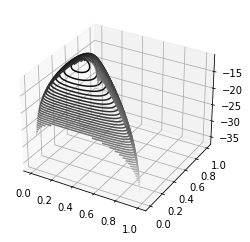
\includegraphics[width=15cm]{homework 2/temp.png}
\end{itemize}

}

\item What is the maximum likelihood estimate of $\theta$ and $\alpha$?
\blue{
\begin{itemize}
    \item  this function is non-concave $log\mathcal{L}_{X}(a,g)=\Sigma_{i=1}^{n}(log(n!)-log(a_i!)-log(g_i!)-log((n-a_i-g_i)!)+a_ilog(\alpha) +g_ilog(\theta) + (n-a_i-g_i)(log(1-\theta-\alpha))$ so i found it more simple to re-write this using a Lagrangian. 
    \item consider the variable $\gamma$ which is the likelihood of a draw.
    \item we can write $log\mathcal{L}_{X}(a,g)=\Sigma_{i=1}^{n}(log(n!)-log(a_i!)-log(g_i!)-log((n-a_i-g_i)!)+a_ilog(\alpha) +g_ilog(\theta) + (n-a_i-g_i)(log(\gamma))$ as long as we add a Lagrange constraint $\Sigma_{i=1}^{n}(log(n!)-log(a_i!)-log(g_i!)-log((n-a_i-g_i)!)+a_ilog(\alpha) +g_ilog(\theta) + (n-a_i-g_i)(log(\gamma))+\lambda(1-\alpha+\theta+\gamma)$
    \item taking the partial with respect to $\theta$ we get $\Sigma_{i=1}^{n}\frac{a_i}{\alpha}-\lambda=0$ yielding $\Sigma_{i=1}^{n}\frac{a_i}{\lambda}=\alpha$
    \item we see similarly that $\Sigma_{i=1}^{n}\frac{g_i}{\lambda}=\theta$ and $\Sigma_{i=1}^{n}\frac{n-a_i-gi}{\lambda}=\gamma$
    \item so here we can see that $1=\alpha+\theta+\gamma=\Sigma_{i=1}^{n}\frac{g_i}{\lambda}+\Sigma_{i=1}^{n}\frac{n-a_i-gi}{\lambda}+\Sigma_{i=1}^{n}\frac{a_i}{\lambda}=1=\frac{N}{\lambda}$ and finally $\lambda=n$
    \item so thus we have $\Sigma_{i=1}^{n}\frac{a_i}{\lambda}=\Sigma_{i=1}^{n}\frac{a_i}{n}=\alpha$ that is our max likelihood alpha is the total number of times anish wins over the total number of trials 
    \item similarly we can see that $\Sigma_{i=1}^{n}\frac{g_i}{\lambda}=\Sigma_{i=1}^{n}\frac{g_i}{n}=\theta$ so that is the ratio of Garry's win over the total number of games
\end{itemize}
}

\item Model the data as realizations from a discrete random variable and compute its empirical pmf. Compare this nonparametric model to the parametric model from the previous questions.  
\blue{
\begin{itemize}
    \item we can model this with the empirical observations from the data so that would be. 
    \item $\alpha_{X}=\frac{\text{number of Anish wins}}{\text{total number of games}}=\frac{2}{10}$ as Anish wins two out of 10 games 
    \item $\theta_{X}=\frac{\text{number of Gary wins}}{\text{total number of games}}=\frac{4}{10}$ as Garry wins four out of 10 games 
    \item this is the same as my solution for the multinomial pdf
\end{itemize}
}
\end{enumerate}

\item (Darts) In a game of darts, a player needs to hit a certain number $k$ times. Assume that all attempts are mutually independent, and that the probability of success in each attempt is $\theta$. Derive the pmf of a random variable representing the number of required attempts.
\blue{
\begin{itemize}
    \item we can kind of model this as something between a geometric and a binomial distribution. 
    \item so first as a modeling assumption. I am going to assume that the player needs to hit k-1 shots, out of his first n-1 shots. and then make the last shot. this makes sense as the if he makes k shots in teh n-1 shots then it would take less than n total shots to hit the number k times and if he does not hit the nth shot then it would take more than n shots to hit k shots. 
    \item so we can model the previous n-1 shots with a binomial. where the likelihood of hitting is theta. so call $\Tilde{a}$ the number of shots he hits in the first n-1 shots. and $P(\Tilde(A)=k-1)=$\begin{pmatrix}n-1\\k-1\end{pmatrix}$\theta^{k-1}(1-\theta)^{((n-1)-(k-1))}$
    \item then call $\Tilde{b}$ a variable with the likelihood of hitting a single shot. modeled with a geometric so $P(\Tilde{b}=1)=\theta$
    \item call $\Tilde{d}$ the total likelihood of it taking you n shots to hit a certain number k times $P(\Tilde{d}=n)=P(\Tilde(A)=k-1)P(\Tilde{b}=1)=$\begin{pmatrix}n-1\\k-1\end{pmatrix}$\theta^{k-1}(1-\theta)^{((n-1)-(k-1))}\theta=$\begin{pmatrix}n-1\\k-1\end{pmatrix}$\theta^{k}(1-\theta)^{n-k}$ 
\end{itemize}
}
\item (Air Traffic)
The tables in \textit{train.csv} and \textit{test.csv} record the numbers of arriving flights at London Heathrow airport every 10 minutes between 18:00 and 19:30 every day. The training and test data are collected from 2010-06-01 to 2010-12-31 and 2011-01-01 to 2011-06-28, respectively. 

\begin{enumerate}
\item Use the training set to estimate the pmf using a parametric model and a nonparametric model. Explain any assumptions you make to choose the parametric model. Plot the nonparametric and  parametric pmfs. 
\blue{
\begin{itemize}
\item It makes most sense to construct a parametric model using the Passion distribution. 
\item first we are going to assume that there exists a fixed rate $\lambda$ at which plains come in. second we are going to assume that if we subdivide our period of observation the likelihood of a plain coming during any specific interval of length n is $\lambda n$. third as n gets sufficiently small, the likelihood of there being two plains during on period of length n approaches zero. finally we assume that the plains are independent of one another. 
\item we know that the pmf of a passion distribution is $P_x (n)=\frac{\lambda^ae^{-\lambda}}{a!
}$  as discussed in class we know the likelihood's function for this is $\mathcal{L}_x(\lambda)=\Pi_{i=1}^{n}P_{x}(x_i)=\Pi_{i=1}^{n}\frac{\lambda^ae^{-\lambda}}{a!
}$ then taking the log of this we get $\Sigma_{i=1}^{n}x_ilog(\lambda)-\lambda-log(x_i!)$ optimizing this yields the max as $\lambda^{*}=\frac{1}{n}\Sigma_{i=1}^{n}x_i$
\item plotting this versus the empirical distribution we get the fol owing graph.
\item 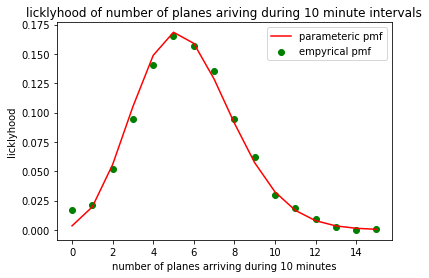
\includegraphics[width=15cm]{homework 2/here.png}
\end{itemize}
 

}
\item Evaluate the performance of your two models on the test set. Compute the root mean square error between the estimated pmfs and the empirical pmf of the test set. Which model performs better?
\blue{
\begin{itemize}
    \item the formula for RMSE is RMSE $\sqrt{\frac{(\Sigma(x_i-\Tilde{x_i})^2}{n}}$
    \item applying this formula we get a parametric RMSE of 0.06589508183337757
    \item and a empirical RMSE of 0.021742471437206635
    \item thus the empirical does better
\end{itemize}
}


\end{enumerate}

\end{enumerate}
\end{document}
